\chapter{Evaluation}
\label{ch:evaluation}

\todo{Chapter intro}

\section{Performance}

\todo{Benchmark SvelteKit without SSR, maybe NextJS Benchmark}

We tested the existing ui5 implementation and the new SvelteKit Implementations, in multiple metrics. We were especially interested in responsiveness to navigation events. To this end we measured first contentful paint (FCP), the time until the page settled, and cumulative layout shift (CLS). Furthermore, we measured time until the page settled, for a navigation from the chauffeur job overview, to the details view of a chauffeur job.

All measurements were conducted on a Lenovo ThinkPad T480, with an Intel Core i7-8550U, and 16 GB RAM, running Windows 11. The measurements where taken using the developer tools of Google Chrome 116.0. The benchmark setup is described in app. \ref{app:benchmark-setup}.

Our measurements (fig. \ref{fig:benchmark}) show, while our implementations took longer to send content to the client, they reduced time until the relevant data is being shown, significantly. These results align with the expected effects of server side rendering, outlined in section \ref{sec:rendering-patterns}. Furthermore, SvelteKit shows significant improvements when navigating between two pages. This is improved even further by SvelteKit's preloading capabilities. In our benchmark, preloading was set to "tap", meaning, the data is being fetched as soon as a \mintinline{html}|mousedown| event is triggered. This data is shown in Pdown nav. While Pup nav shows the time from, when a click event is fired.  

\begin{figure}
    \centering
    \begin{tikzpicture}
        \begin{axis}[
                ybar,
                bar width=.7cm,
                width=.9\textwidth,
                height=.5\textwidth,
                legend style={at={(0,1)},
                    anchor=north west,legend columns=1},
                legend cell align={left},
                symbolic x coords={TTFB,FCP,CP,Nav},
                xtick=data,
                enlarge x limits={0.15},
                nodes near coords,
                nodes near coords align={vertical},
                ymin=0,ymax=4000,
                ylabel={duration (ms)},
            ]
            \addplot table[x=type,y=ui5]{\benchmarkdata};
            \addplot table[x=type,y=sk-fs]{\benchmarkdata};
            \addplot table[x=type,y=sk-fe]{\benchmarkdata};
            \legend{UI5, SvelteKit Full Stack, SveleKit FE-only}
        \end{axis}
    \end{tikzpicture}
    \label{fig:benchmark}
    \caption{Benchmark Results for TTFB, FCP, CP and Nav}
\end{figure}

Levlin, has shown, that SvelteKit can provide significant improvements in certain areas over frameworks like react and angular.  

\section{Bundle Size}

Smaller, but no data yet... fuck all 

\section{Something else}

% \begin{itemize}
%     \item SEO
%     \item Community support
%     \item DX
%     \item ecosystem
%     \item performance
% \end{itemize}

\section{Experience}

% \begin{itemize}
%     \item Both approaches (full stack and frontend only) worked great
%     \item advantage of full-stack: 
%     \item no API definition required
%     \item reuse of models between UI and business logic or even type inference
% \end{itemize}

In this section we give our personal experience developing with SvelteKit in an attempt to reason about SvelteKit's expected developer experience. As we noted in \Cref{sec:methodology}, providing a heuristic analysis of SvelteKit's DX is out of scope.

In our experience both discussed implementations (full stack in SvelteKit and SvelteKit only for frontend) enabled an efficient and pleasant development experience. Especially the full stack approach significantly reduced overhead, because models could be reused between client and server and communication between server and client happened transparently.

% \begin{itemize}
%     \item Concise / Intuitive Syntax
%     \item reduction of client-server waterfalls
%     \item SPA/SSR/SSG with single framework
%     \item clear data flow (load function $\rightarrow$ svelte, svelte $\rightarrow$ action)
% \end{itemize}

\subsection{Project Setup}

SvelteKit provides a command line utility to create new projects (\Cref{fig:project-setup}). This utility provides options to configure TypeScript for type checking, ESLint\footnote{\url{https://eslint.org/}} for code linting, Prettier\footnote{\url{https://prettier.io/}} for code formatting, as well as Vitest\footnote{\url{https://vitest.dev/}} and Playwright\footnote{\url{https://playwright.dev/}} for testing. 


% \begin{itemize}
%     \item Fast, \mintinline{bash}|npm cgeate svelte@latest|
%     \item missing out-of-the-box features: form validation/parsing
% \end{itemize}

\begin{figure}
    \centering
    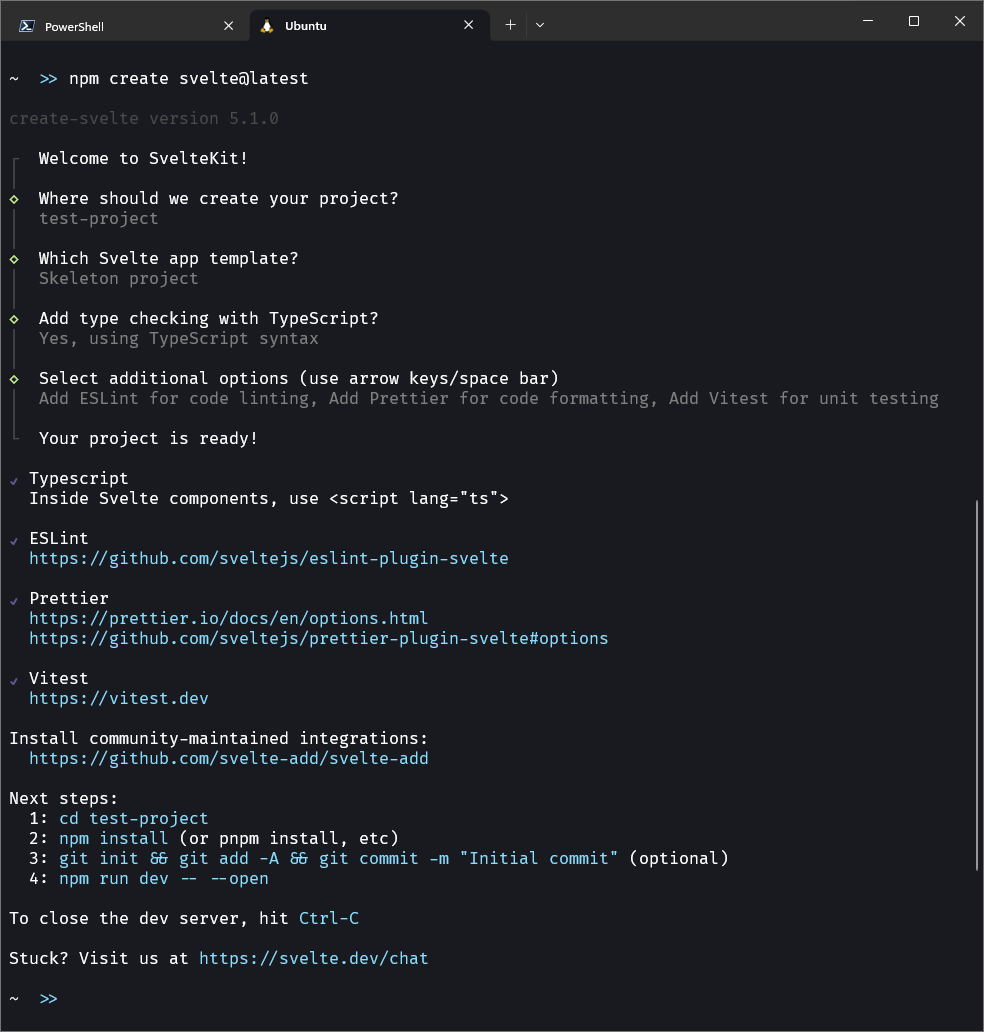
\includegraphics[width=.95\linewidth,trim={0 15cm 0 1.5cm},clip]{assets/sveltekit-project-setup}
    \caption{Process for creating a new SvelteKit project}
    \label{fig:project-setup}
\end{figure}

\subsection{Syntax}

We experienced Svelte's syntax as easy to grasp. This is because Svelte's syntax closely adheres to HTML with some added features for templating and reactivity.

Svelte's decision to reuse assignment operators for reactivity, not only makes for a less verbose, but also more intuitive syntax. Something, something code snippet:

\begin{myminted}{svelte}{Svelte}
<script>
    let count = 0;
</script>

<button on:click={() => (count++)}>+</button>
\end{myminted}

\begin{myminted}{jsx}{React}
import { useState } from 'react';

export function Component() {
    const [count, setCount] = useState(0);

    return <button onClick={() => setCount(c => c + 1)}>+</button>
}
\end{myminted}

This example clearly shows how Svelte simplifies a common use case, by utilizing its compiler based approach.

Simple Store API:
\begin{myminted}[escapeinside=||]{svelte}{}
<script>
    import { writable } from 'svelte/store';

    const todos = writable([]);
</script>

<button on:click={() => todos.}>add Todo</button>
{#each |\$|todos as todo}
    <div>{todo.text}</div>
{/each}
\end{myminted}

Simple Reactive Statements:
\begin{myminted}[escapeinside=||]{svelte}{}
<script>
    let count = 0;
    |\$|: doubled = count * 2;
</script>
\end{myminted}

\subsection{Library Interoperability}

\begin{itemize}
    \item Nice interop because Svelte is close to vanilla HTML/JS/CSS
    \item Svelte Code is valid HTML/JS/CSS Syntax $\rightarrow$ Tools work out of the box (e.g Prettier, ESLint)
\end{itemize}


\subsection{Routing}
SvelteKit decided to integrate a filesystem-based routing system. This comes with some inherit advantages and disadvantages. Probably the biggest advantages is, that this approach makes immediately clear what the purpose of a file is. Especially for simple cases this routing system works with no overhead and makes it possible to work very fast, when adding new routes. But some problems become apparent in more complex examples. Projects with a large amount of routes will inevitably have many files with the same name. In our experience this could make it harder sometimes to use IDE search functions to quickly navigate between many files, because searching most of the time returned more than one \mintinline{bash}|+page.svelte| or \mintinline{bash}|+page.js| file. Furthermore, solutions to some problems can cause a lot of file changes in a version control system. During our implementation efforts, we found the need to wrap multiple routes in a layout group. This meant, all files hat to be moved to a new subdirectory. This caused a lot of noise in the version control system for a change that was simple in nature. With a declarative routing solution the same problem could have been solved by simple changing the router configuration.

It has also to be noted that this filesystem-based approach to routing makes it effectively impossible to split a singular SvelteKit application into multiple smaller projects. Because routing is strictly bound to the filesytem, it is only possible to configure routing in the root project.

% \begin{itemize}
%     \item Good: It is immediately clear which file does what
%     \item Bad: a lot of \mintinline{svelte}|+page|-files
%     \item bad: Simple Changes can suddenly cause a lot of file moves: e.g. adding a custom layout around a group of routes.
% \end{itemize}

\subsection{Clear data flow}

Clear direction: +page.server.js $\rightarrow$ +page.js $\rightarrow$ +page.svelte.

\subsection{Svelte works best with plain HTML}

As described in \Cref{sec:implementation-ui}, the implementation was required to follow the SAP Fiori Design Guidelines. To this end we tried using both UI5 web components and a plain CSS classes approach using SAP Fundamental Styles. In either case we decided to create a library of Svelte components that wraps the actual UI utility. This decision was made to reduce the amount of boilerplate code and repetition required to use some UI elements. Furthermore, this decision made it easier to migrate from UI5 web components to fundamental styles, because only the Component library hat to be changed. 



% In our implementation we experimented with different approaches to structuring our UI-code

% \begin{itemize}
%     \item Most directives do not work on Components (use:, class:, style: )
%     \item Scoped styles means, it is annoying to pass down locally defined CSS-classes to children.
%     \item But, Tailwind CSS can make things better (because everything is defined globally anyway).
% \end{itemize}


% \subsection{Cases where Svelte is bad}
% While SvelteKit can provide an improved development experience, it does not come without its flaws. During out study we identified multiple areas where SvelteKit caused problems, or could become a paint point in larger projects.

% \begin{itemize}
%     \item Centralized load function (compared to RSC's, load where needed)
%     \item Things Which require node.js server (e.g. cron, websockets)
%     \item Big data sets, which need to be shared between routes (virtuelle-fabrik)
%     \item Style is scoped per default, thus it is annoying to pass classes to child component (improved with tailwind, because everything is global)
%     \item Differences between client renderer and server renderer
%     \item No best practices yet
%     \item Problems with Svelte's Custom fetch
% \end{itemize}

\subsection{Universal vs. Server Load Functions}


% - problems with universal
% - SvelteKit fetch weird
% - auth more complicated
% - 

\subsection{Reactivity Pitfalls}

While Svelte's reactivity is overall very intuitive, it nonetheless has some pitfalls.

Svelte's reactive blocks work by analyzing all local variables that are used in this block. If one of those variables changes, the reactive block is rerun. But, this only works if the dependent variable is used directly in the reactive block. In cases where the dependency is used in a function for example, the dependency cannot be analyzed and therefore will not trigger executions of the reactive block:

\begin{myminted}[escapeinside=||, autogobble]{svelte}{}
<script>
    let count = 1;

    let doubled;
    |\$|: calcDoubled();

    function calcDoubled() {
    doubled = count * 2;
    }
</script>

<button on:click={() => (count++)}>+</button>
<div>{count} * 2 = {doubled}</div>
\end{myminted}

In this example, the function \mintinline{svelte}|calcDoubled|, calculates the value of \mintinline{svelte}|double| in correspondence to \mintinline{svelte}|count|. But because \mintinline{svelte}|count| is not directly used in the reactive statement, the reactive statement will not trigger when \mintinline{svelte}|count| is updated.

\subsubsection{Centralized load function}

SvelteKit's architecture enforces that all asynchronous data has to be acquired inside a pages load function, for it to be available during server side rendering. This provides a clean and easy to understand flow for simple implementations. But it can increase complexity in cases where a single isolated component has to be reused in multiple different routes.

One could for example imagine a simple component which displays a Twitter feed, which has to be used in multiple places. Given following file hierarchy:

\begin{myminted}{html}{}
routes/
  a/
    +page.js
    +page.svelte
  b/
    +page.js
    +page.svelte
  TwitterComponent.svelte
\end{myminted}

Both route a and b need to use the twitter component. The way to implement this in SvelteKit would be to fetch the data in the load function of both routes and pass it to the twitter component as a prop:

\begin{myminted}{js}{\string{a,b\string}/+page.js}
export async function load({ fetch }) {

    const twitterFeed = (await fetch('/api/twitterfeed')).json();

    return {
        twitterFeed,
        // other page data...
    }
}

\end{myminted}

\begin{myminted}{svelte}{\string{a,b\string}/+page.svelte}
<script>
    import TwitterComponent from '../TwitterComponent.svelte';

    export let data;
</script>

<TwitterComponent feed={data.twitterFeed} />
<!-- other page markup... -->
\end{myminted}

\begin{myminted}{svelte}{TwitterComponent.svelte}
<script>
    export let feed
</script>

{#each feed as tweet}
    <!-- ... -->
{/each}
\end{myminted}

This pattern needs to be repeated for each route that wants to use the twitter component. This not only results in unnecessary code duplication, but can also cause problems later in a project's lifecycle. If the twitter component is to be removed later on, it is imaginable that one of the fetch calls is left in by accident, because the data fetching is detached from where the data is actually used, thus causing unnecessary traffic.

Other approaches circumvent this problem by coupling data fetching more closely to its usage. For example, a similar implementation using React Server Components could look something like this:

\begin{myminted}{jsx}{TwitterComponent.jsx}
export async function TwitterComponent() {
    const twitterFeed = await (await fetch('/api/twitterfeed')).json();

    return <>
        {twitterFeed.map(tweet => (
            // ...
        ))}
    </>
}
\end{myminted}

\begin{myminted}{jsx}{\string{a,b\string}/page.jsx}
import TwitterComponent from '../TwitterComponent';

export async function Page() {
    return <>
        <TwitterComponent />
        { /* other page markup... */ }
    </>
}
\end{myminted}

With this approach, the Twitter component becomes truly isolated from the page, because it can fetch its own data. We expect this architecture to scale better in large applications, than SvelteKit's centralized load function.


\subsection{Deployment}

SvelteKit provides first-class adapters that automate creating production deployments for various hosting providers such as Vercel\footnote{\url{https://vercel.com/}}, Netlify\footnote{\url{https://www.netlify.com/}}, Cloudflare Pages\footnote{\url{https://pages.cloudflare.com/}}, and Cloudflare Workers\footnote{\url{https://workers.cloudflare.com/}}. Furthermore, adapters exist to create standalone NodeJS server, or generate a static bundle that can be served from a simple file-base web server. Beyond this, a wide range of community plugins exist which further extend the range of platforms, SvelteKit can be deployed to. This means that SvelteKit generally supports great flexibility for deployment with comparatively little effort.  

But, this wide range of supported platforms creates some shortcomings. SvelteKit does mostly not implement features that require platform specific functionality. One such feature would be a hook that is executed when the application shuts down. This can sometimes be required for example to close open connections. While this can be easily worked around in a NodeJS environment, by using \mintinline{js}|process.on('sigint', ...)|, other features are not added this easily. 

Websockets are another feature that is currently not supported out of the box, because some providers such as Vercel have no support for websockets yet \cite{noauthor_vercel_nodate}. While it is possible to add websocket support to the NodeJS platform this is not possible without shortcomings. By default, the NodeJS adapter creates an entry point that starts a web server to host all handlers required by SvelteKit. It is possible to forego this entry point and instead write a custom server that uses the handlers directly. In this way it is possible to create a web server that uses websockets. But, this approach only works for the production build, in development, another workaround is required that works with hot-module replacement. Furthermore, a separate 

% todo: SvelteKit wants to be a serverless framework\cite{noauthor_expose_nodate} 


\subsection{Stability}

% \begin{itemize}
%     \item Svelte 2 to 3 was big change
%     \item Svelte 5, while being maintained for 2 major versions, will also come with migrations.
% \end{itemize}

Version 1.0 of SvelteKit released only recently in December 2023 \cite{team_announcing_2022}, thus it is not possible to tell how stable the APIs of the framework will be going forward. Svelte on the other hand has reached its fourth major version. So far, version 3 made changes to its API, which caused a need for manual migrations. 


\subsection{Future of Svelte}

On 20. September 2023, The Svelte team gave a first preview of the next major new API planned for version 5 of Svelte, called runes. Runes are a set of compiler instructions that replace the system of reactivity currently used in Svelte. With runes, Reactivity becomes more explicit. Instead of every top level variable in a svelte file being reactive by default, state that should be reactive has to be marked with the \mintinline{svelte}|$state| rune:

\begin{myminted}[escapeinside=||]{svelte}{}
<script>
    let count = |\$|state(0);
</script>
\end{myminted}

While initially being more verbose, this has multiple advantages. Firstly, this syntax is more explicit, clearly marking which variable is reactive and which is not. Secondly, this syntax is not limited to the top-level of a svelte file, further, it will even be possible to place state-runes in JavaScript files. This will make it easier to move out state in to separate files. Where as before, stores were required to place state in separate files, with this new syntax it will be possible to use the same syntax in svelte-files and in js-files.

Furthermore, Svelte 5 introduces two runes that replace the \mintinline{svelte}|$:| syntax, \mintinline{svelte}|$derived| and \mintinline{svelte}|$effect|:

\begin{myminted}[escapeinside=||]{svelte}{}
<script>
    let count = |\$|state(0);

    const doubled = |\$|derived(count * 2);

    |\$|effect(() => {
        console.log(`new value of count: ${count}`);
    })    
</script>
\end{myminted}
\s{$}


% svelte likely wont go away